\subsection{Corporate Identity}

What is the first thing you should think about, when you see our logo? Why did we use these colors? Why did we decide to take this font? 

These are just a few questions related to the corporate identity. It determinates how the project team presents itself to the public. Within the corporate identity document everything regarding public appearance can be defined. This could contain the behaviour to the public, as well as communication, philosophy, design, language and much more. 

In case of OctoTagger it was decided to just take care of the design part from the corporate identity, the corporate design. This document contains our design-guidelines for the website. This includes the colors used for the logo and other images, the background colors, the font and the logo itself. 

The challenge at developing a corporate design is to always keep the user in mind. How does the user think? What does he want to see? It's important to attract a potential user and catch his attention. The website is the first thing every potential user gets confronted with, so it has to send the right signals. Colors are great triggers for emotions and feelings making them a powerful tool for the writer of the corporate design. However, the proper combination of the colors is at least as important as the colors themselves. 

The logo design should not be neglected. It's an essential part of the corporate design. The challenge is to design a logo that provides a distinctive look but keeping it as simple as possible at the same time. 

\subsection{Background of the name OctoTagger}

In the beginning there was just the idea for the product, an file organisation software. Afterwards the name OctoTagger was born. The intention behind that name was indeed an octopus and it's ability to handle several actions at the same time, due to his eight arms. In this point OctoTagger and octopuses share similarities. OctoTagger is also able to handle multiple files at the same time. So the octopus became our mascot and the corporate design was developed out of this idea later. 

\subsection{Corporate Design for OctoTagger}
\subsubsection{Colors}

The colors were the first part of the corporate design to be defined. Because of our mascot the octopus, it was decided to chose colors related to the living environment of octopuses which is the sea. We picked several shades of green and blue to fit this scheme. These tones became our primary colors which means that they are used most of the time. However, just using this colors would be too monotonous, so a secondary color set was added. It contains some complementary colors of the primary colors and is just used rarely.

\paragraph{Primary Colors} \hspace{0pt} \\

\definecolor{primary_1}{RGB}{118,178,76}
\definecolor{primary_2}{RGB}{49,201,175}
\definecolor{primary_5}{RGB}{130,227,166}
\definecolor{primary_3}{RGB}{23,197,200}
\definecolor{primary_6}{RGB}{123,215,213}
\definecolor{primary_4}{RGB}{59,177,216}

\begin{tabular}{ c  c  c  c }
\#76B24C & \crule[primary_1]{3cm}{3cm} & \#31C9AF & \crule[primary_2]{3cm}{3cm} \\
\#17BBC8 & \crule[primary_3]{3cm}{3cm} & \#3BB1D8 & \crule[primary_4]{3cm}{3cm} \\
\#82E3A6 & \crule[primary_5]{3cm}{3cm} & \#7BD7D5 & \crule[primary_6]{3cm}{3cm} \\ 
\end{tabular}

\paragraph{Secondary Colors} \hspace{0pt} \\

\definecolor{secondary_1}{RGB}{255,193,0}
\definecolor{secondary_2}{RGB}{255,140,62}
\definecolor{secondary_3}{RGB}{255,92,62}

\begin{tabular}{ c  c  c  c }
\#FFC100 & \crule[secondary_1]{3cm}{3cm} & \#FF8C3E & \crule[secondary_2]{3cm}{3cm} \\
\#FF5C3E & \crule[secondary_3]{3cm}{3cm} \\
\end{tabular}

\paragraph{Background Colors} \hspace{0pt} \\

\definecolor{background_1}{RGB}{240,240,240}
\definecolor{background_2}{RGB}{193,200,197}

\begin{tabular}{ c  c }
\#F0F0F0 & \crule[background_1]{6cm}{3cm} \\
\#C1C8C5 & \crule[background_2]{6cm}{3cm} \\
\end{tabular}\\



During the color-planing process it was decided to include two different background colors into the corporate design. The first one is a light gray shade which reduces the contrast between the background and the content above it. It is used as background color on the entire website. The second color consists of a much darker shade of gray. It's mainly used to create a second background layer over the first background. 

\subsubsection{Fonts}

As font, the DejaVu font family is used on the website. It follows the general guidelines of the OctoTagger website by being straight and modern. Below an example of the DejaVu font can be seen.\\


\includegraphics[scale=0.30]{images/font.png}


\subsubsection{Logo}

\paragraph{First drafts} \hspace{0pt} \\

The first concept for the logo of OctoTagger was the combination of an octopus and a folder symbol. These two elements were brought together seamlessly. However, it did not measure up to our expectations as the octopus was hardly recognizable. 

The sketch can be seen in the following image:

\begin{center}
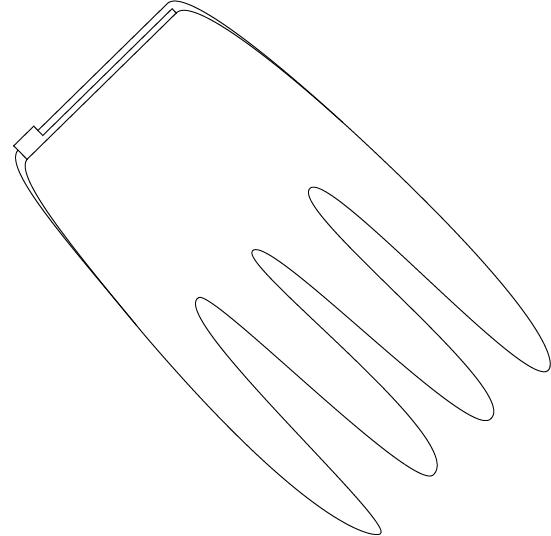
\includegraphics[scale=0.30]{images/logo_v01.png}
\end{center}

The second draft was an enhanced version of the first one. It was tried to keep it more even and linear, furthermore colors were added for the first time. This version of the logo consists of two parts, the file symbol on the top, symbolizing the body of the octopus, and four tentacles below it.

The image below shows the second sketch:

\begin{center}

\includegraphics[scale=0.30]{images/logo_v02.png}
\end{center}

This sketch became even more abstract then the first one and we got some negative feedback. Later it was replaced by an improved version, our actual logo.

\subsubsection{Current logo}

For the final version of the logo, the first concept was adopted and the idea of a folder symbol in our logo was dropped. It was decided to just include the octopus into the logo. This octopus has four visible tentacles on the front and four more in the background. At the end of these arms tags are attached.

The outcome can be seen below:


\begin{center}

\includegraphics[scale=0.30]{images/logo.png}
\end{center}

A version including the project name is also available:

\begin{center}

\includegraphics[scale=0.30]{images/logo_text.png}
\end{center}